%% ****** Start of file aiptemplate.tex ****** %
%%
%%   This file is part of the files in the distribution of AIP substyles for REVTeX4.
%%   Version 4.1 of 9 October 2009.
%%
%
% This is a template for producing documents for use with 
% the REVTEX 4.1 document class and the AIP substyles.
% 
% Copy this file to another name and then work on that file.
% That way, you always have this original template file to use.

%\documentclass[aip,jap,numerical,preprint]{revtex4-1}
\documentclass[twocolumn,secnumarabic,amssymb, nobibnotes, aps, pra]{revtex4}
\newcommand{\revtex}{REV\TeX\ }
\newcommand{\classoption}[1]{\texttt{#1}}
\newcommand{\macro}[1]{\texttt{\textbackslash#1}}
\newcommand{\m}[1]{\macro{#1}}
\newcommand{\env}[1]{\texttt{#1}}
\newcommand{\norm}[1]{\lVert#1\rVert}
\setlength{\textheight}{9.5in}

\usepackage{caption}
\usepackage{amsmath}
\usepackage{graphicx}
\usepackage{booktabs}
\usepackage{color}
\usepackage{enumerate}
\providecommand{\e}[1]{\ensuremath{\times 10^{#1}}}

\DeclareCaptionType{mycapequ}[][List of equations]
\captionsetup[mycapequ]{labelformat=empty}

%\draft % marks overfull lines with a black rule on the right

\begin{document}

%Title of paper
\title{Magnetic Torque and the Dipole Moment
% \large{Methods of experimental physics} \\ 
 %\normalsize{PHYS 413}
 }

% repeat the \author .. \affiliation  etc. as needed
% \email, \thanks, \homepage, \altaffiliation all apply to the current
% author. Explanatory text should go in the []'s, actual e-mail
% address or url should go in the {}'s for \email and \homepage.
% Please use the appropriate macro foreach each type of information

% \affiliation command applies to all authors since the last
% \affiliation command. The \affiliation command should follow the
% other information
% \affiliation can be followed by \email, \homepage, \thanks as well.
\author{Jason Morgan}
%\email[]{Your e-mail address}
%\homepage[]{Your web page}
%\thanks{}
%\altaffiliation{}
\affiliation{Department of Physics, Old Dominion University, Norfolk VA 23529}



\date{March 27, 2014}


\begin{abstract}
The dipole moment $\vec{\mu}$ of a magnet is a measure of the strength of the magnet and creates magnetic torque when in the presence of an external magnetic field.  This lab will measure the $\vec{\mu}$ of a magnet using three different methods.  Experiment one will measure $\vec{\mu}$ by applying a gravitational torque opposing the magnetic torque.  The second experiment uses the period of small amplitude oscillation to make the measurement of $\vec{\mu}$.  Experiment three calculates $\vec{\mu}$ by measuring the precessional angular velocity.  
\end{abstract}

\maketitle
\section{Introduction}

The magnetic dipole moment $\vec{\mu}$ of a permeant magnet is a measure of a magnet’s strength.   $\mu$ is modeled on a current loop where $\mu = IA$ with I being the current in Amperes and A being the area of the loop in $m^2$.  When placed in an external magnetic field the potential energy associated with the dipole is $U = - \vec{\mu} \cdot \vec{B}$.  Therefore the potential energy of the system is minimum whent $\vec{\mu}$ is aligned with $\vec{B}$ and is a maximum when $\vec{\mu}$ is anit aligned with $\vec{B}$.  The magnet will experience a restoring toruqe when $\mu$ in not aligned with the external magnetic field.  This torque on a current loop or magnet is equal to: 

\begin{mycapequ}[!ht]
\begin{equation}
\vec{\tau} = \vec{\mu} \times \vec{B}
\label{torque}  %label the equation
\end{equation}  
\caption{Where $\vec{\mu}$ is the dipole moment and $\vec{B}$ is the external magnetic field}
\end{mycapequ}
The three experiments in this lab rely on the effects of this magnetic torque on the dipole to measure  $\vec{\mu}$.  

\section{Theory}
\subsection{Magnetic torque equals gravitational torque}
The first experiment conducted in this lab equates the magnetic torque on a rod and weight to the magnetic torque.  When the sum of these torques is zero the rod and cue will be rotationally stable and the weight will not move when carefully released.

\begin{mycapequ}[!ht]
\begin{equation}
\vec{\mu} \times \vec{B} = \vec{r} \times m\vec{g}  = \norm{\vec{\mu}} \norm{\vec{B}}sin(\theta) = m\norm{\vec{r}}\norm{\vec{g}}sin(\theta)
\label{sumoftorque}   %label the equation
\end{equation}  
\caption{Where m is the mass of the weight, $\vec{r}$ is the position of the weight with respect to the center of the cue and $\vec{g}$ is the acceleration due to gravity.}
\end{mycapequ}

Since the angle between $\vec{\mu}$ and $\vec{B}$ and the angle between $\vec{r}$ and $\vec{g}$ are the same, the dependency on the angle $\theta$ is eleminated and the equation can be reduced to:

\begin{equation}
\norm{\vec{r}} = \frac{\norm{\vec{\mu}} \norm{\vec{B}}}{m\norm{\vec{g}}}
\label{magnitudeofr}   %label the equation
\end{equation}  

Equation \ref{magnitudeofr} allows for the calulation of $\norm{\vec{\mu}}$ given the length of the rod, the mass of the weight, the acceleration due to gravity and the strength of the external magnetic field.  The value of $\norm{\vec{\mu}}$ will be the slope of the line when $\norm{\vec{r}}$ is plotted vs the $\norm{\vec{B}}$ times the mass of the weight and the magnitude of the acceleration due to gravity.

\subsection{Harmonic oscillation of a sperical pendulum}

A magnetic dipole that is displaced by an angle $\theta$ form an external magnetic field $\vec{B}$ it will experience a torque that acts against the displacement which is given by equation \ref{torque}.  This leads to the following differential equation:

\begin{mycapequ}[!ht]
\begin{equation}
\norm{\vec{\mu}} \norm{\vec{B}} sin(\theta) = -\frac{dL}{dt} = -I\frac{d^2\theta}{dt^2}
\label{eom1}   %label the equation
\end{equation}  
\caption{I is the moment of inertia of the cue ball and $\theta$ is the angle of displacement}
\end{mycapequ}

This can be made into a linear differential by limiting the displacement and using the small angle approximation which state that $sin(\theta) \approx \theta$.  This approzimation is good to within 1\% for angles less that $\approx$ 14 degrees \cite{mcalister1}.  This results in the following differential equation that is solvable via analytic means:

\begin{equation}
I\frac{d^2\theta}{dt^2} - \norm{\vec{\mu}} \norm{\vec{B}} \theta = 0
\label{eom2}   %label the equation
\end{equation}  

Equation \ref{eom2} has a solution of the form $\theta(t) = Acos(\omega t)$ where $\omega$ is the angular velocity and A is a constant.  Substituting into equation \ref{eom2} and solveing for $\omega^2$ we get 

\begin{equation}
\omega^2 = \frac{\norm{\vec{\mu}}\norm{\vec{B}}}{I}
\label{omega}   %label the equation
\end{equation} 

The period of oscillation is given by that $T = \frac{2\pi}{\omega}$.  Squaring this equation and substituting for $\omega^2$ from \ref{omega} we get

Equation \ref{T2} allows for the calulation of $\norm{\vec{\mu}}$ given the moment of inertia of the cue ball, the period of oscillation and the strength of the external magnetic field.  The value of $\norm{\vec{\mu}}$ will found using the relation:

\begin{equation}
\norm{\vec{\mu}} = \frac{4\pi^2}{slope}
\label{eg:slope}   %label the equation
\end{equation} 

where slope is the slope of the line that results when $T^2$ is plotted vs  $\frac{I}{\norm{\vec{B}}}$.

\subsection{Precessional motion of a spinning sphere}

The last experiment performed uses the precessional motion of a spinning sphere to measure $\norm{\vec{\mu}}$.  When a spinning magnetic dipole is exposed to an external magnetic field, it will experience a torque that changes the angular momentum in the direction of the torque.  This causes the the cue to precess in the direction of the torque due to it's large angular momentum due to spinning.  The equation of motion for this precession is:

\begin{equation}
\vec{\mu} \times \vec{B} = \frac{dL}{dt}
\label{precess1}   %label the equation
\end{equation} 

\begin{equation}
\frac{dL}{dt} = \Omega_p\norm{\vec{L}}sin(\theta)
\label{precess2}   %label the equation
\end{equation} 


where $\Omega_p$ is the precessional frequency.  Equating queation \ref{precess1} and \ref{precess2} and simplifing we get

\begin{equation}
\Omega_p = \frac{\norm{\vec{\mu}}}{\norm{\vec{L}}} \norm{\vec{B}}
\label{precess3}   %label the equation
\end{equation} 

Equation \ref{precess3} allows for the calulation of $\norm{\vec{\mu}}$ given precessional frequency, the angular momentum of spin and the strength of the external magnetic field.  The value of $\norm{\vec{\mu}}$ will be the slope of the line when $\Omega_p$ is plotted vs the $\frac{\norm{\vec{B}}}{\norm{\vec{L}}}$.


\section{Experimental setup and procedures}

The set of for all three experiments includes a helmholtz coil, a cue ball with a magnetic dipole in the center, an air bearing and a power supply.  The helmholtz coil supplies a constange magnetic field at it's center to create a magnetic torque on the magnetic dipole in the center of the cue ball.  The air bearing make the effects of friction negligable in the cue ball, allowing it to rotate freely.  There is a rod and weight for performing the measurment of $\norm{\vec{\mu}}$ by equating the magnetic torque to the gravetational torque.  There is also a strobe light be deternining the angular momentum of the cue ball for the experiment for precessional motion.

The first step was to measure all constant parameters for all the experiments.  The following quantities were measured: the mass of the cue ball, the mass ot the weight, the diameter of the cue ball.  We then calculated the moment of inertia of the cue ball.  The value are reported in table \ref{tab:params}. 

\begin{table} [h]  % Capital letters stronger suggestion
\caption{Constant Parameter Measurments and Calculations}      %title of the table     
\centering              % centering table
\begin{tabular}{ccc} % creating four columns (c stands for ceneter, r for right, l for left)
\hline\hline %inserting double-line
  Measurement & Result   \\
\hline % inserts single-line
Mass of cue ball & 0.1420 $\pm$ 0.0001 kg \\
Diameter of cue ball & 0.0537 $\pm$ 0.0001 m  \\
Mass of weight & 1.30 $\pm$ 0.01 g  \\
Moment of Inertia & $4.095 x 10^{-5}$ $\pm$ 0.01 g  \\



\hline % inserts single-line
\end{tabular}
\label{tab:params}
\end{table}

\subsection{Magnetic torque equals gravitational torque}

First the power supply was turned on.  The air supply to the air bearing was then turned on. The weight was placed at a distance of 4.00 $\pm$ 0.05 cm from the bottom of the rod.  The rod was then inserted into the handle of the cue ball until in stopped.  The cue ball was placed on the air bearing.  Next the DB current was slowly turned on with the magnetic field direction switch set to the up direction.  The current was continuously adjusted until the rod and weight could be carefully released and remain motionless at a 90 degree angle (with zero degrees being straight up.)  Getting the rod to remain motionless was difficult as any slight motion would cause the rod to move.  Given the precision of the current measurement it was found to be most reliable to adjust the current until a slight almost imeasurable adjustment of greater or lesser current would cause the rod to consistently move in one direction or the other when released.  The distance $\norm{\vec{r}}$ of the weight form the center of mass of the cue ball as well as the current at which the torques on the weight balanced was then recorded.  This process was then repeated each time the weight was moved farther from the center of mass of the cue ball.  

\subsection{Harmonic oscillation of a sperical pendulum}

The power supply was turned on.  The air supply to the air bearing was then turned on.  The rod and weight were removed from the handle on the cue ball.  The current to the helmholtz coil was set to 0.95 $\pm$ 0.05 A.  The handle of the cue ball was then displaced from the verticle by a small angle (less than 14 degrees).  After a couple of oscillation of the handle, a stopwatch was started at the beginning of a period.  The stopwatch was stopped when 20 oscillations were reached.  The time in seconds was recorded in a table along with the current.  This process was repeated increasing the current by 0.25 $\pm$ 0.05 A each time until 2.00 $\pm$ .05 A was reached.  The then the current was increased in increments of 0.05A until a current of 4.00 $\pm$ 0.05 A was attained.  


\subsection{Precessional motion of a spinning sphere}

The helmholtze coil was covered with a cardboard box to improve the visibility of the strobe light.  The power supply was turned on.  The air supply to the air bearing was then turned on.  The strobe light was then turned on and set to a frequency of 5 Hz.  The handle of the cue ball was then displaced from the vertical be an angle less than 90 degrees pointing towards the strobe light.  The cue ball was then made to spin around the axis of the handle.  When the white dot on the tip of the handle appeared in a constant position, the current to the helmholtz coil was quickly set to 1.00 $\pm$ 0.05 A and a stopwatch was started.  When the handle cmpleted one complete revolution, the stopwatch was stoped.  The value if the current and time in seconds to complete on revolution was then recored.  This process was then repeated while increasing the the current in increments of 0.5 $\pm$ 0.05 A until and 4.0 $\pm$ 0.05 A was reached. The process was then repeated for the same current values and the results were averaged.

\section{Results and Discussion}
\subsection{Magnetic torque equals gravitational torque}

The data was plotted (Fig. \ref{fig:grav}) to show the magnitude of the gravitational torque as a function of the external magnetice field.  This results in a straight line with $\norm{\vec{\mu}}$ as the slope of the line. Plotting and fitting the data using the R language gave a value for $\norm{\vec{\mu}}$ of 0.419 $\pm$ 0.008 $A * m^2$.

\subsection{Harmonic oscillation of a sperical pendulum}

The data was plotted (Fig. \ref{fig:oscillatory}) to show time squared as a function of current over the external magnetic field.  This provides a straight line with a slope of $3.8\times 10^-3 \pm 2 \times 10^-4$ by plotting the data using the R language.  $\norm{\vec{\mu}} $ is then found using Eq. \ref{eg:slope} to be $0.425 \ pm 0.001 A * m^2$


\subsection{Precessional motion of a spinning sphere}

The data was plotted (Fig. \ref{fig:oscillatory}) to show the precessional angular velocity in radians per second vs the external magnetic field divided by the spin angular momentum.  This provides a straight line where the slope is equal to $\norm{\vec{\mu}} $ when plotted using the R language.  The value $\norm{\vec{\mu}} $ is found to be $0.42 \pm 0.02 A*m^2$. 

\section{Conclusion}

The magnetic torque experiments were great experiments to perform.  The measurement of the value of $\norm{\vec{\mu}}$ was made by three different methods and came out with the same values given the error ranges.  There was not an explicit value given for the $\norm{\vec{\mu}}$ for the magnet in the cue ball we were using so the error in our measurements cannot be stated definitively. 


\newpage
\begin{figure} [b]  %htb stands for here, top and bottom and gives a suggestion to Latex where to place the graph
\begin{center}
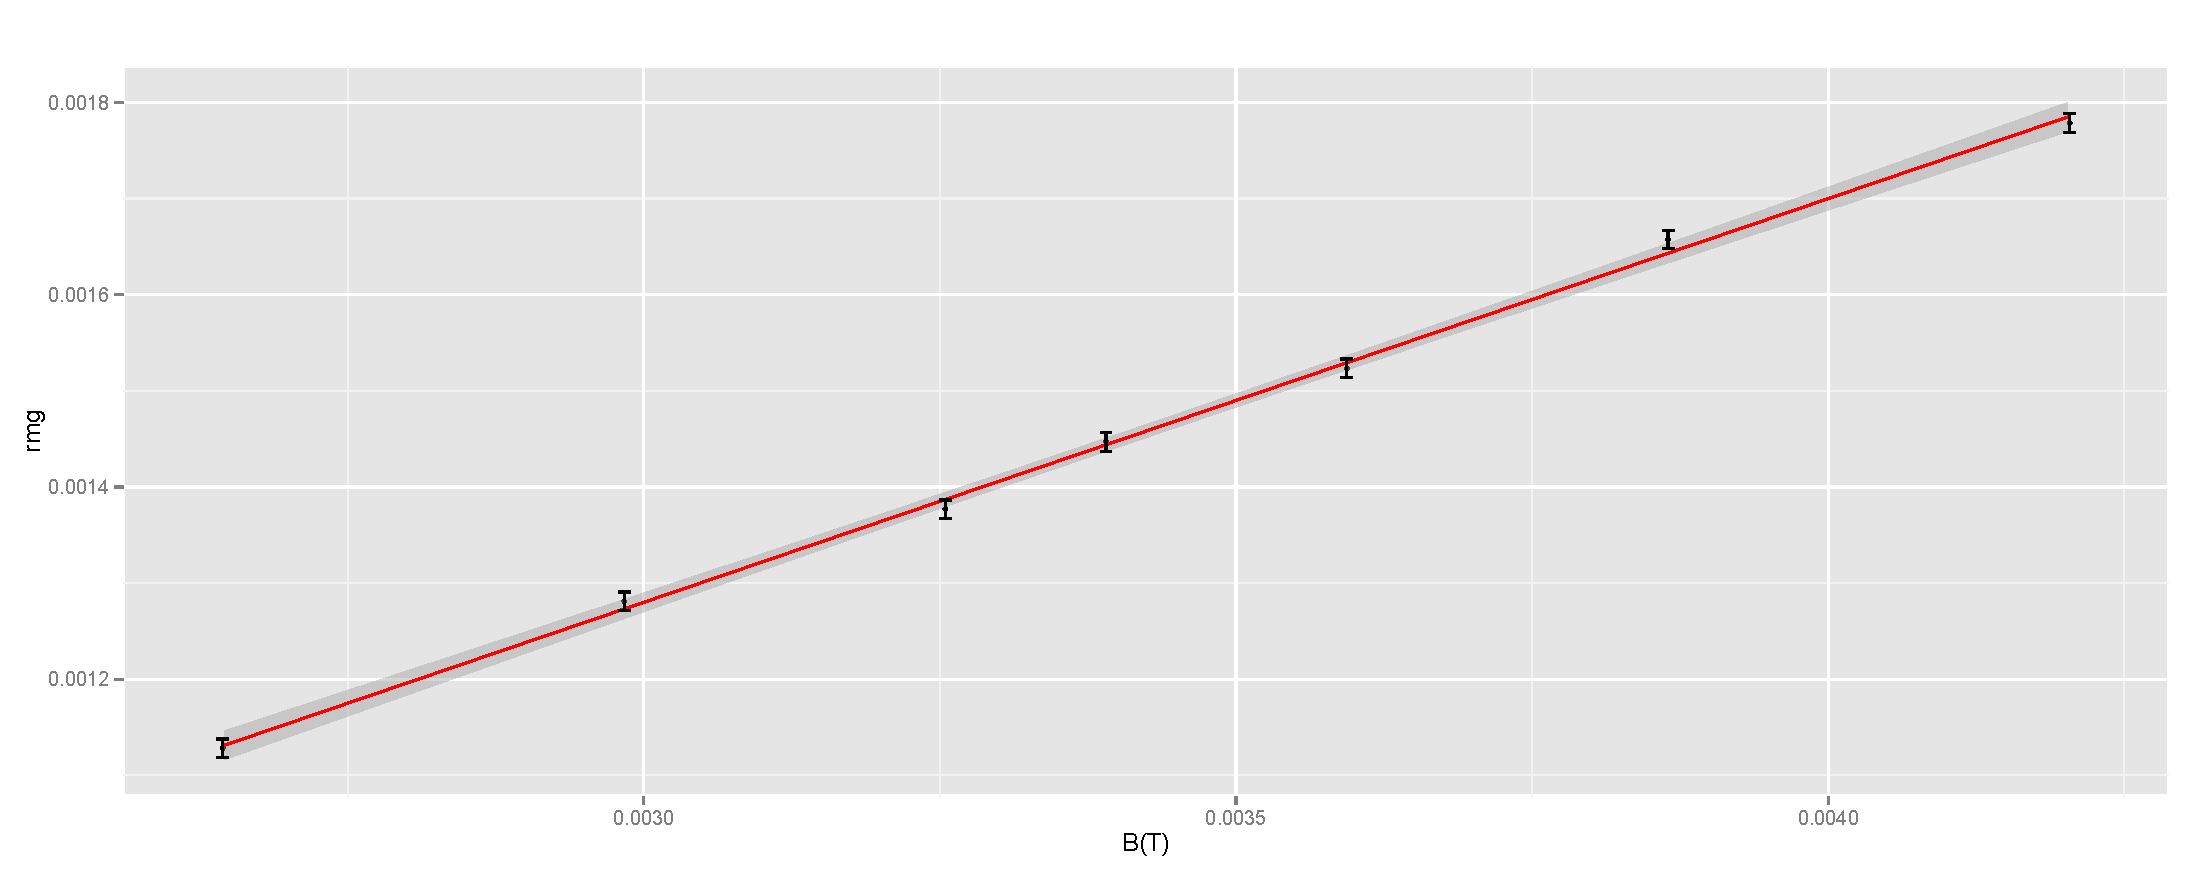
\includegraphics[scale=.5]{grav.pdf} 
\end{center}
\caption{rmg as a function of the external magnetic field. $\norm{\vec{\mu}}$ 0.419 $\pm$ 0.008 $A * m^2$.  $R^2$ = 0.998}
\label{fig:grav}
\end{figure}


\begin{figure} [b]  %htb stands for here, top and bottom and gives a suggestion to Latex where to place the graph
\begin{center}
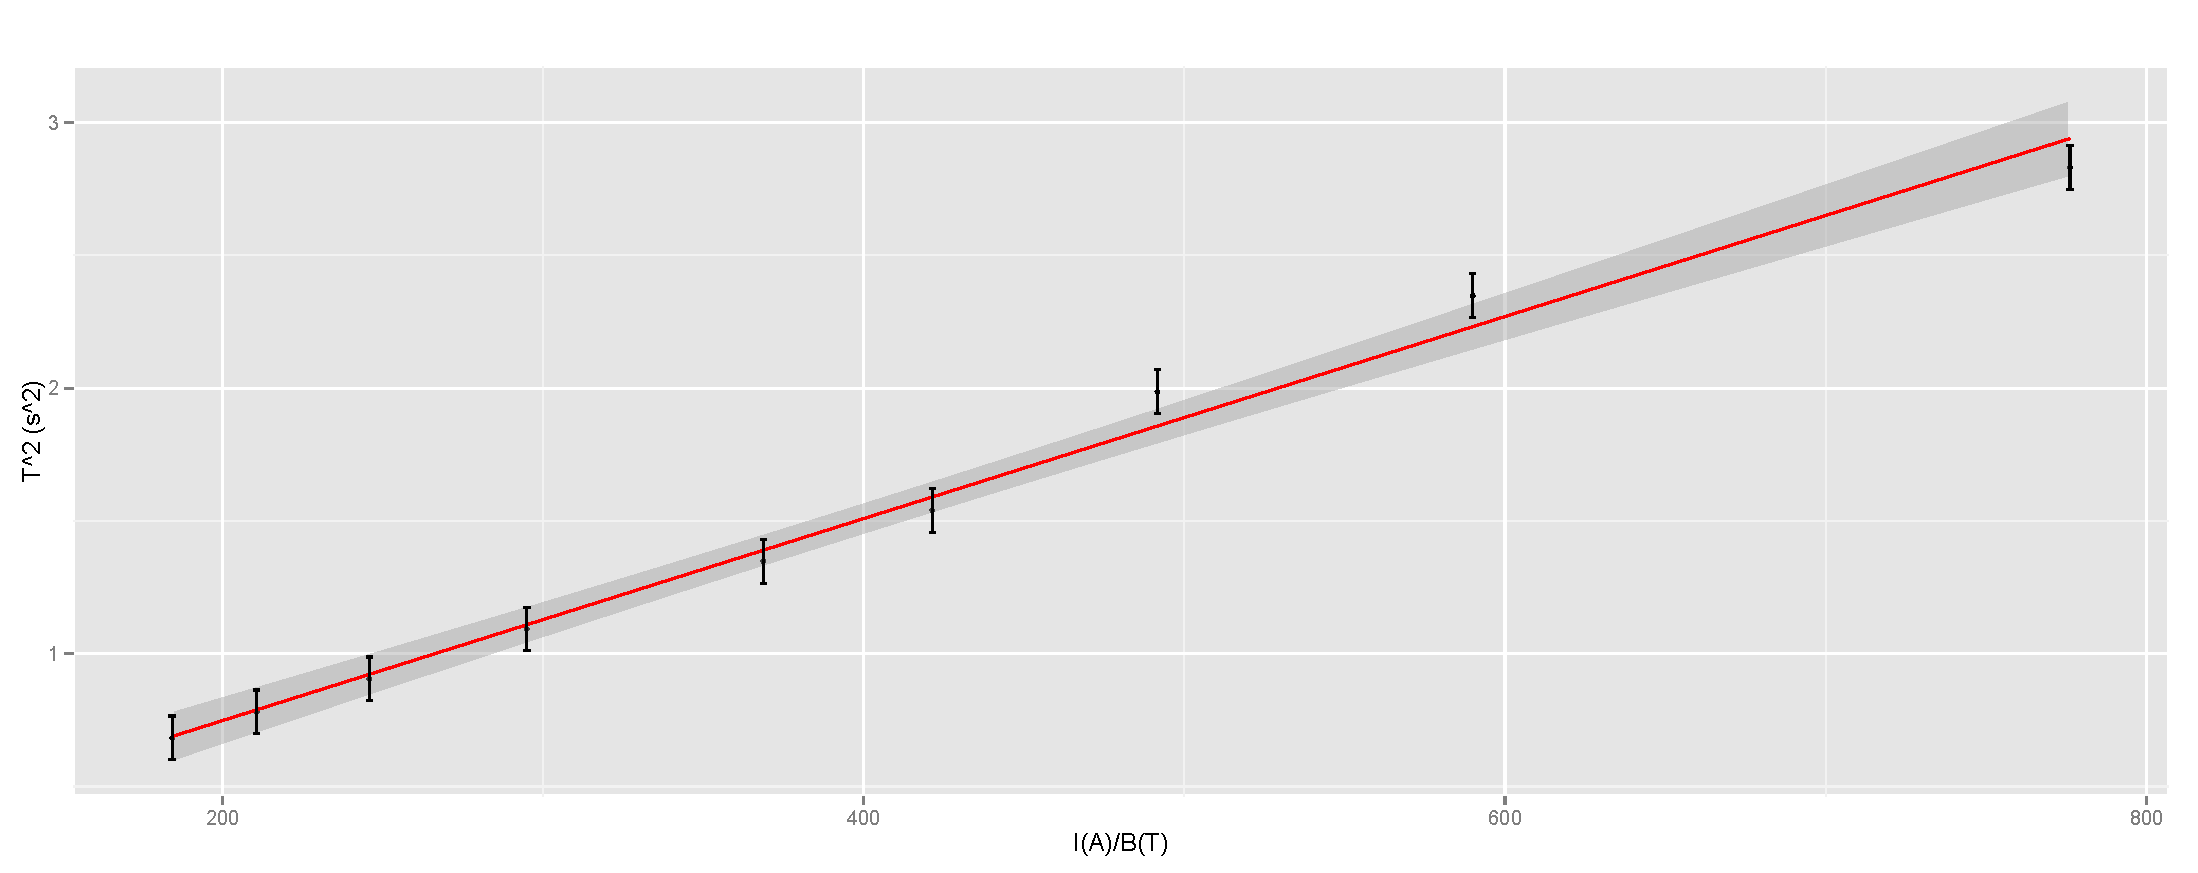
\includegraphics[scale=.5]{oscillatory.pdf} 
\end{center}
\caption{$T^2$ as a function of the external magnetic field. $\norm{\vec{\mu}}$ 0.425 $\pm$ 0.001 $A * m^2$.  $R^2$ = 0.989}
\label{fig:oscillatory}
\end{figure}


\begin{figure} [b]  %htb stands for here, top and bottom and gives a suggestion to Latex where to place the graph
\begin{center}
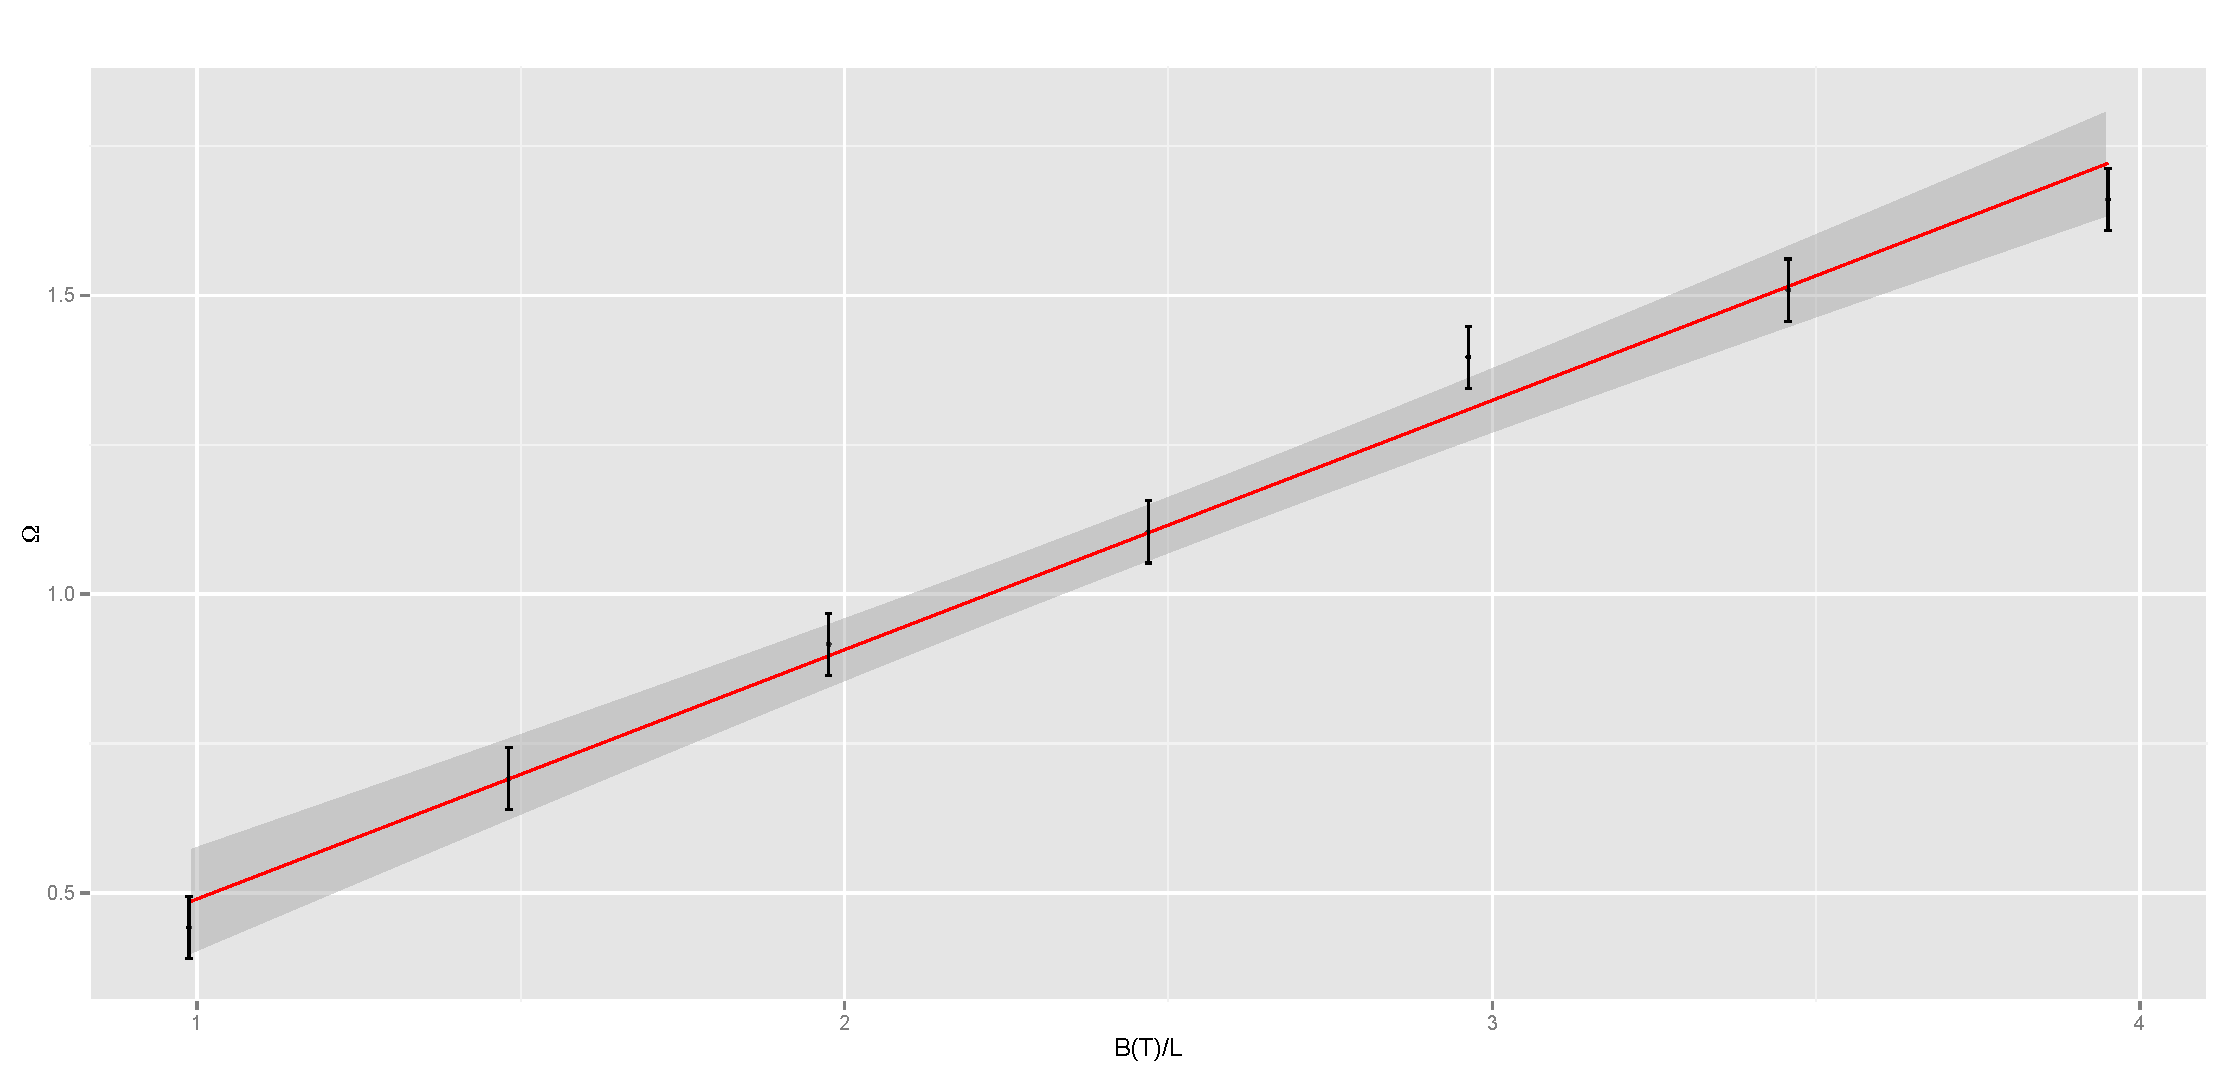
\includegraphics[scale=.5]{precession.pdf} 
\end{center}
\caption{$\Omega$ in radians per second as a function of the external magnetic field divided by the angular momentum. $\norm{\vec{\mu}}$ 0.42 $\pm$ 0.02 $A * m^2$.  $R^2$ = 0.989}
\label{fig:precession}
\end{figure}



%Write down references
%-----------------------------------
\begin{thebibliography}{5}
\bibitem{mcalister1} Wikipedia. "Small-angle approximation.", \textit{Wikipedia}, Wikimedia Foundation, 03 Sept. 2014. Web. 27 Mar. 2014.
\bibitem{mcalister2} TEACHSPIN. "Magnetic Torque.", \textit{TeachSpin}, Tri-Main, Web. 21 April. 2014.

\end{thebibliography}

\end{document}

%
% ****** End of file aiptemplate.tex ******
